\documentclass[10pt]{standalone}
\usepackage{amsmath}
\usepackage{pgf,tikz}
\usepackage{mathrsfs}
\usetikzlibrary{arrows}
\pagestyle{empty}
\begin{document}
	
		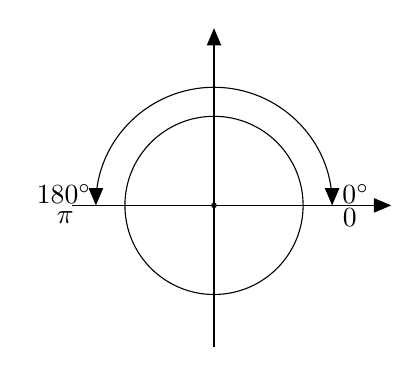
\begin{tikzpicture}[>=triangle  45,x=1.5cm,y=1.5cm]
		\coordinate (C) at (0,0);
		\coordinate (A) at (1.5,0);
		\coordinate (B) at (-1.2,0);
		\coordinate (AA) at (0.0,-1.2);
		\coordinate (CC) at (0.0,1.5);

		
			\draw[->] (AA) - -(CC);
		\draw[->] (B) - -(A);
		\draw [<->] (1.0,0.0) arc(0:180:1);
		\node (A1) at (1.2,0.1) {$0^\circ$};
		\node (A2) at (-1.27,0.1) {$180^\circ$};
	\node (B1) at (1.15,-0.1) {$0$};
	\node (B2) at (-1.26,-0.1) {$\pi$};
		\node[draw, circle, inner sep=0.8cm] (a) at (C) {};
\draw (C) circle  (0.8 pt);
\filldraw[black](C);
		\end{tikzpicture}
\end{document}